\section{Resolución Problema 3}
La busqueda de la distancia entre dos puntos y la verificación de si se encuentran dentro de una circunferencia en Java es posible crear un programa que realice estos cálculos y determine la ubicación de los puntos con respecto a una circunferencia proporcionada por el usuario.
Para calcular la distancia entre dos puntos, se utiliza la fórmula de la distancia. Esta fórmula nos permite obtener una medida precisa de la distancia en un plano, teniendo en cuenta las coordenadas x,y de los puntos.
El programa calculará la distancia entre los puntos utilizando la fórmula mencionada y luego utilizará una estructura condicional para determinar si los puntos se encuentran dentro de la circunferencia o fuera de ella, en función del radio ingresado.
De esta manera, el programa en Java proporcionará una solución eficiente y precisa para determinar la ubicación de los puntos en relación con la circunferencia, basándose en el cálculo de la distancia y el uso de una estructura condicional.
\subsection{\textbf{Descripción del problema:}}
\begin{enumerate}
    \item El problema tiene como objetivo determinar si un punto $T$ con coordenadas $(x_{2}, y_{2})$ se encuentra dentro del área de una circunferencia. El usuario proporcionará las coordenadas $(x_{1}, y_{1})$ del centro de la circunferencia, las coordenadas $(x_{2}, y_{2})$ del punto $T$, y el radio $r$. El proceso implica utilizar la ecuación de distancia entre dos puntos y presentar la respuesta resultante.
\end{enumerate}
\begin{figure}[h!]
    \centering
    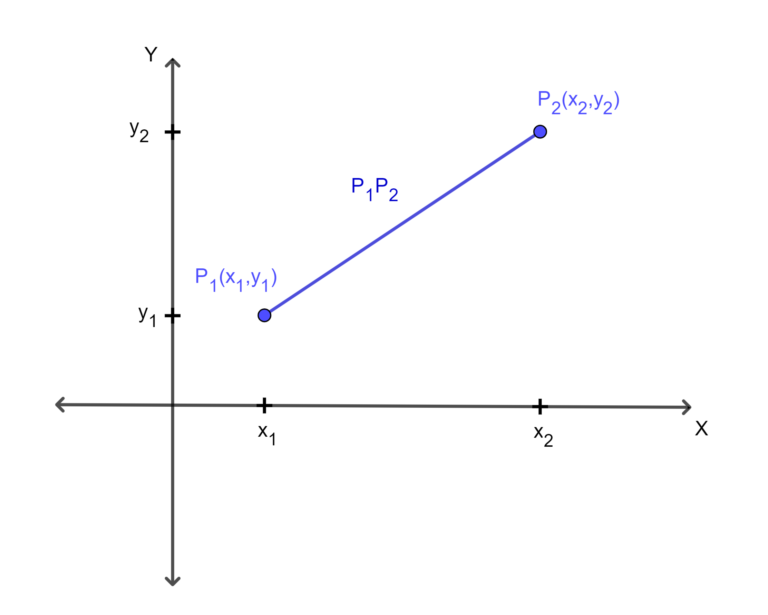
\includegraphics[width=1\linewidth]{LaTeX//latex-imagenes/Distancia_entre_dos_puntos-2-768x615.png}
    \caption{La distancia entre dos puntos.}
    \label{fig:enter-label}
\end{figure}
\subsection{\textbf{Definición de solución:}}
La solución consiste en evaluar si un punto $T$ con coordenadas $(x_{2}, y_{2})$ está dentro del área de una circunferencia con centro en $(x_{1}, y_{1})$ y radio $r$. Para ello se utiliza la fórmula de la distancia entre dos puntos y se compara la distancia calculada con el radio $r$ de la circunferencia:
    \begin{equation}
        \text{distancia} = \sqrt{ (x_2 - x_1)^2 + (y_2 - y_1)^2 }
    \end{equation}
    
    \begin{enumerate}
        \item Si la distancia es mayor que el radio $r$, el punto $T$ está fuera de la circunferencia.
        \item Si la distancia es igual al radio $r$, el punto $T$ está en el borde de la circunferencia.
        \item Si la distancia es menor que el radio $r$, el punto $T$ está dentro del área de la circunferencia.
    \end{enumerate}
\subsection{\textbf{Diseño de la solución:}}
\begin{enumerate} 
    \item Solicitar al usuario las coordenadas del centro de la circunferencia $(x_{1}, y_{1})$, las coordenadas del punto $T$ $(x_{2}, y_{2})$, y el radio $r$.
    
    \item Calcular la distancia entre el centro y el punto $T$ utilizando la fórmula de distancia entre dos puntos:
    \begin{equation}
        \text{distancia} = \sqrt{ (x_2 - x_1)^2 + (y_2 - y_1)^2 }
    \end{equation}

    \item Verificar si la distancia calculada es mayor que el radio $r$:
    \begin{enumerate}
        \item Si es mayor, el punto $T$ está fuera de la circunferencia.
    \end{enumerate}
    
    \item Verificar si la distancia calculada es igual al radio $r$:
    \begin{enumerate}
        \item Si es igual, el punto $T$ está en el borde de la circunferencia.
    \end{enumerate}

    \item Verificar si la distancia calculada es menor que el radio $r$:
    \begin{enumerate}
        \item Si es menor, el punto $T$ está dentro del área de la circunferencia.
    \end{enumerate}
    
    \item Presentar el resultado al usuario.
    
\end{enumerate}

\begin{figure}[h!]
    \centering
    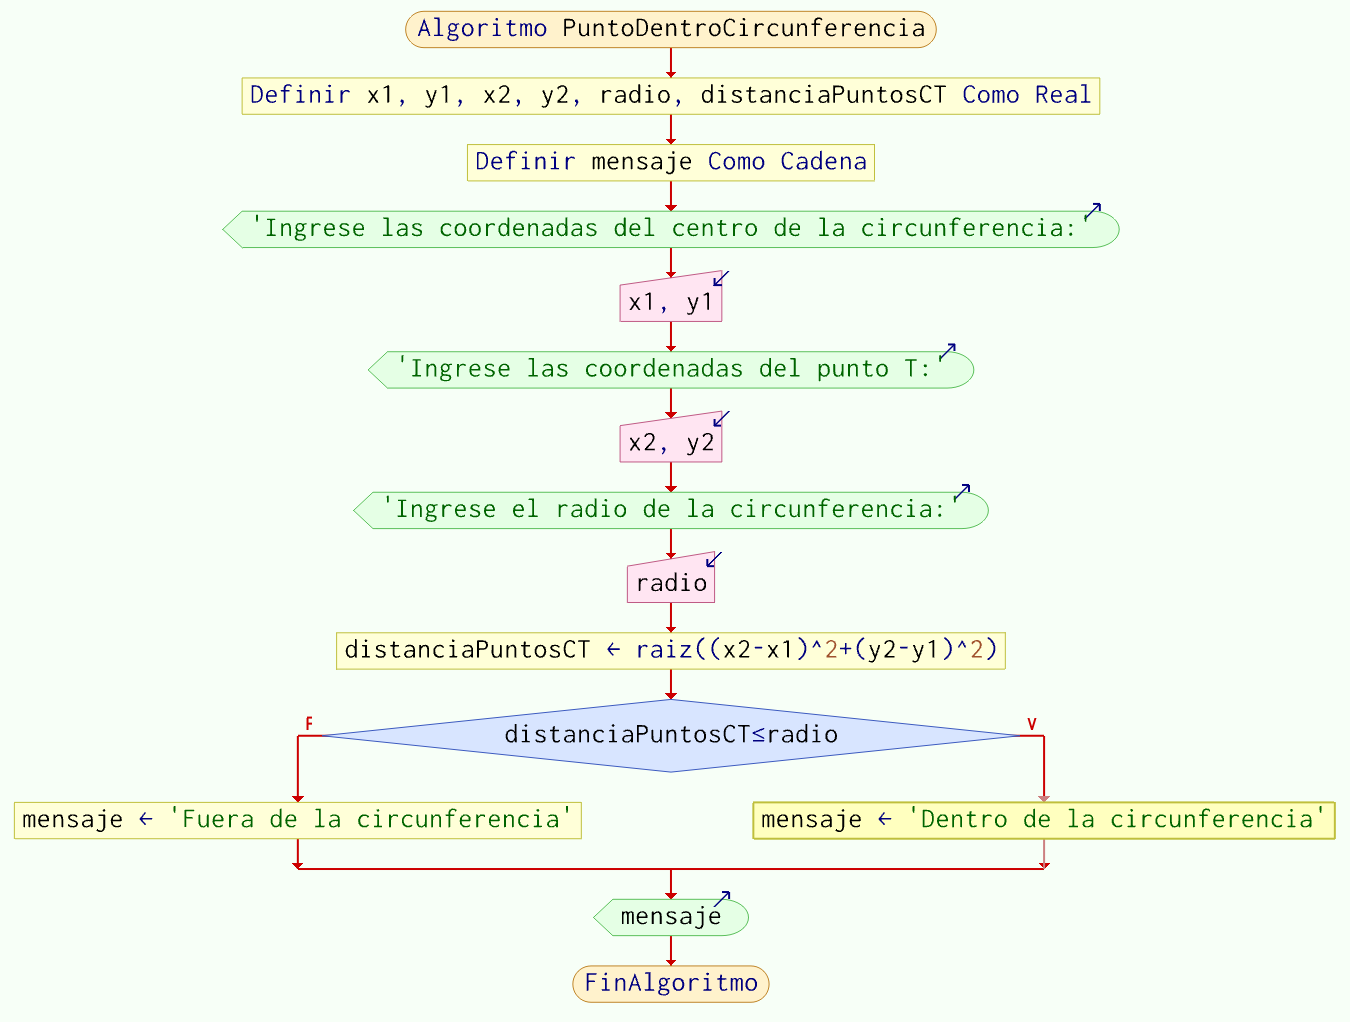
\includegraphics[width=1\linewidth]{LaTeX//latex-imagenes/Captura de pantalla 2023-11-23 150737.png}
    \caption{Diagrama de flujo.}
    \label{fig:enter-label}
\end{figure}
\subsection{\textbf{Desarrollo de la solución:}}
Programa en Java.
\newline
    
Se utiliza un objeto Scanner para obtener datos de entrada desde la consola.\\ Se solicitan al usuario las coordenadas del centro de una circunferencia (punto C), el radio de la circunferencia y las coordenadas de un punto T. \\
    Los valores ingresados se almacenan en arreglos de cadenas de caracteres y se cierra el objeto Scanner para liberar recursos.
\newline
    \begin{javaCode}
        Scanner datos = new Scanner(System.in);
        System.out.println("Ingresa las coordenadas del centro de una circunferencia (punto C) separado por una coma (x,y):");
        String[] puntoC = (datos.nextLine()).split(",");
        System.out.println("Ingresa el radio de la circunferencia:");
        float radio = datos.nextFloat();
        datos.nextLine();
        System.out.println("Ingresa los valores de \"x\" y \"y\" del punto a evaluar (punto T) separado por una coma (x,y):");
        String[] puntoT = (datos.nextLine()).split(",");
        datos.close();
    \end{javaCode} 
    % Bloque de Procedimientos
Se convierten las coordenadas del punto C y del punto T de cadenas de caracteres a números enteros (int). \\
    Luego, se utiliza la fórmula de la distancia para calcular la distancia entre los puntos C y T, almacenando el resultado como un número de punto flotante (float).
    
    \begin{javaCode}
        int xc = Integer.parseInt(puntoC[0].trim());
        int yc = Integer.parseInt(puntoC[1].trim());
        int xt = Integer.parseInt(puntoT[0].trim());
        int yt = Integer.parseInt(puntoT[1].trim());
        float distanciaPuntosCT = (float)Math.sqrt(Math.pow(xt-xc, 2) + Math.pow(yt-yc, 2));
    \end{javaCode}
    
    % Bloque de Salida de Datos
    Se declara una cadena de caracteres vacía llamada "mensaje". \\
    Se utiliza una estructura condicional para determinar la posición relativa del punto T con respecto a la circunferencia y asignar un mensaje correspondiente. Finalmente, se imprime el mensaje en la consola.
    
    \begin{javaCode}
        String mensaje = "";
        if (distanciaPuntosCT > radio) {
            mensaje = "El punto T("+xt+","+yt+") esta fuera de la circunferencia";
        } else if (distanciaPuntosCT == radio) {
            mensaje = "El punto T("+xt+","+yt+") esta en la circunferencia";
        } else {
            mensaje = "El punto T("+xt+","+yt+") esta dentro de la circunferencia";
        }
        System.out.println(mensaje);
    \end{javaCode}
\subsection{\textbf{Depuración y pruebas:}}
\begin{figure}[h!]
    \centering
    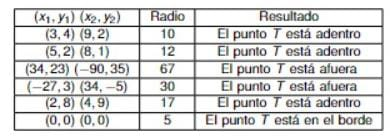
\includegraphics[width=1\linewidth]{c8e8865c-0fa3-4437-b97a-0e67eb053d1f.jpg}
    \caption{Tabla de pruebas}
    \label{fig:enter-label}
\end{figure}